\documentclass{article}

\usepackage{hyperref}
\usepackage{fancyhdr}
\usepackage{braket}
\usepackage{extramarks}
\usepackage{amsmath}
\usepackage{amsthm}
\usepackage{amsfonts}
\usepackage{tikz}
\usepackage[plain]{algorithm}
\usepackage{algpseudocode}
\usepackage{mathtools}
\usepackage{graphicx}
\graphicspath{ {./Images/} }

\DeclarePairedDelimiter\abs{\lvert}{\rvert}%
\DeclarePairedDelimiter\norm{\lVert}{\rVert}%

\makeatletter
\let\oldabs\abs
\def\abs{\@ifstar{\oldabs}{\oldabs*}}
%
\let\oldnorm\norm
\def\norm{\@ifstar{\oldnorm}{\oldnorm*}}
\makeatother

\newcommand*{\Value}{\frac{1}{2}x^2}%

\usetikzlibrary{automata,positioning}

%
% Basic Document Settings
%

\topmargin=-0.45in
\evensidemargin=0in
\oddsidemargin=0in
\textwidth=6.5in
\textheight=9.0in
\headsep=0.25in

\linespread{1.1}

\pagestyle{fancy}
\lhead{\hmwkAuthorName}
\chead{\hmwkClass\ (\hmwkClassInstructor\ \hmwkClassTime): \hmwkTitle}
\rhead{\firstxmark}
\lfoot{\lastxmark}
\cfoot{\thepage}

\renewcommand\headrulewidth{0.4pt}
\renewcommand\footrulewidth{0.4pt}

\setlength\parindent{0pt}

%
% Create Problem Sections
%

\newcommand{\enterProblemHeader}[1]{
    \nobreak\extramarks{}{Problem \arabic{#1} continued on next page\ldots}\nobreak{}
    \nobreak\extramarks{Problem \arabic{#1} (continued)}{Problem \arabic{#1} continued on next page\ldots}\nobreak{}
}

\newcommand{\exitProblemHeader}[1]{
    \nobreak\extramarks{Problem \arabic{#1} (continued)}{Problem \arabic{#1} continued on next page\ldots}\nobreak{}
    \stepcounter{#1}
    \nobreak\extramarks{Problem \arabic{#1}}{}\nobreak{}
}

\setcounter{secnumdepth}{0}
\newcounter{partCounter}
\newcounter{homeworkProblemCounter}
\setcounter{homeworkProblemCounter}{1}
\nobreak\extramarks{Problem \arabic{homeworkProblemCounter}}{}\nobreak{}

%
% Homework Problem Environment
%
% This environment takes an optional argument. When given, it will adjust the
% problem counter. This is useful for when the problems given for your
% assignment aren't sequential. See the last 3 problems of this template for an
% example.
%
\newenvironment{homeworkProblem}[1][-1]{
    \ifnum#1>0
        \setcounter{homeworkProblemCounter}{#1}
    \fi
    \section{Problem \arabic{homeworkProblemCounter}}
    \setcounter{partCounter}{1}
    \enterProblemHeader{homeworkProblemCounter}
}{
    \exitProblemHeader{homeworkProblemCounter}
}

%
% Homework Details
%   - Title
%   - Due date
%   - Class
%   - Section/Time
%   - Instructor
%   - Author
%

\newcommand{\hmwkTitle}{Homework\ \#11}
\newcommand{\hmwkDueDate}{April 14, 2020}
\newcommand{\hmwkClass}{Physics 926}
\newcommand{\hmwkClassTime}{}
\newcommand{\hmwkClassInstructor}{Professor Ken Bloom}
\newcommand{\hmwkAuthorName}{\textbf{Robert Tabb}}

%
% Title Page
%

\title{
    \vspace{2in}
    \textmd{\textbf{\hmwkClass:\ \hmwkTitle}}\\
    \normalsize\vspace{0.1in}\small{Due\ on\ \hmwkDueDate\ at 5pm}\\
    \vspace{0.1in}\large{\textit{\hmwkClassInstructor\ \hmwkClassTime}}
    \vspace{3in}
}

\author{\hmwkAuthorName}
\date{}

\renewcommand{\part}[1]{\textbf{\large Part \Alph{partCounter}}\stepcounter{partCounter}\\}

%
% Various Helper Commands
%

% Useful for algorithms
\newcommand{\alg}[1]{\textsc{\bfseries \footnotesize #1}}

% For derivatives
\newcommand{\deriv}[1]{\frac{\mathrm{d}}{\mathrm{d}x} (#1)}

% For partial derivatives
\newcommand{\pderiv}[2]{\frac{\partial}{\partial #1} (#2)}

% Integral dx
\newcommand{\dx}{\mathrm{d}x}

% Alias for the Solution section header
\newcommand{\solution}{\textbf{\large Solution}}

% Probability commands: Expectation, Variance, Covariance, Bias
\newcommand{\E}{\mathrm{E}}
\newcommand{\Var}{\mathrm{Var}}
\newcommand{\Cov}{\mathrm{Cov}}
\newcommand{\Bias}{\mathrm{Bias}}

\begin{document}

\maketitle
*In addition to the lecture notes, the following resources were used to better understand the material:\\
\url{https://arxiv.org/ftp/arxiv/papers/1511/1511.06752.pdf}\\

\pagebreak

\begin{homeworkProblem}
	Show that
	\[
		P(\nu_1 \rightarrow \nu_2) = \sin^22\theta\sin^2\frac{\Delta m_{12}^2L}{4E}
	\]
	for a two neutrino system in which the mixing matrix is
	\[
		U=\begin{pmatrix}
		\cos\theta & \sin\theta \\
		-\sin\theta & \cos\theta
		\end{pmatrix}
	\]
	and $\Delta m_{12}^2=m_1^2-m_2^2$
	\\
	\\
	\textbf{Solution}
	\\
	\\
	Equation (7) from the lecture gives us a good starting point. This equation is an approximation which is valid when mass is small, which in this case it is
	\[
		P(\nu_1 \rightarrow \nu_2) = \abs{\sum_i U_{1i}^* U_{2i} e^{-im_i^2L/2E}}^2
	\]
	Using this equation as a starting point, we can plug in the given values of $U$ and explicitly do the sum.
	\[
		\begin{split}
		\abs{\sum_i U_{1i}^* U_{2i} e^{-im_i^2L/2E}}^2 =& \left[ \sum_i U_{1i}^* U_{2i} e^{-im_i^2L/2E} \right] \left[ \sum_j U_{1j}^* U_{2j} e^{-im_j^2L/2E} \right]^* \\
		=& \left[ \sum_i U_{1i}^* U_{2i} e^{-im_i^2L/2E} \right] \left[ \sum_j U_{2j}^* U_{1j} e^{im_j^2L/2E} \right] \\
		\sum_i U_{1i}^* U_{2i} e^{-im_i^2L/2E} =& \cos\theta(-\sin\theta) e^{-im_1^2L/2E} + \sin\theta\cos\theta e^{-im_2^2L/2E} \\
		=& -\cos\theta\sin\theta e^{-im_1^2L/2E} + \cos\theta\sin\theta e^{-im_2^2L/2E} \\
		=& \cos\theta\sin\theta \left( e^{-im_2^2L/2E} - e^{-im_1^2L/2E} \right) \\
		\sum_j U_{2j}^* U_{1j} e^{im_j^2L/2E} =& -\sin\theta\cos\theta e^{im_1^2L/2E} + \cos\theta\sin\theta e^{im_2^2L/2E} \\
		=& \cos\theta\sin\theta \left( e^{im_2^2L/2E} - e^{im_1^2L/2E} \right) \\
		\end{split}
	\]
	\[
		\begin{split}
		\left[ \sum_i U_{1i}^* U_{2i} e^{-im_i^2L/2E} \right] \left[ \sum_j U_{2j}^* U_{1j} e^{im_j^2L/2E} \right] =& \cos^2\theta\sin^2\theta \left( e^{-im_2^2L/2E} - e^{-im_1^2L/2E} \right) \left( e^{im_2^2L/2E} - e^{im_1^2L/2E} \right) \\
		=& \cos^2\theta\sin^2\theta \left( 2 - e^{i(m_1^2-m_2^2)L/2E} - e^{-i(m_1^2-m_2^2)L/2E} \right) \\		
		=& \cos^2\theta\sin^2\theta \left( 2 - 2Re\left[e^{i(m_1^2-m_2^2)L/2E}\right] \right) \\
		=& 2\cos^2\theta\sin^2\theta \left( 1 - \cos\frac{\Delta m_{12}^2L}{2E}  \right)
		\end{split}
	\]
	From here, use the trig identity: \(1-cos\theta = 2\sin^2\frac{\theta}{2}\) and then $2\cos\theta\sin\theta = \sin2\theta$:
	\[
		\begin{split}
		\left[ \sum_i U_{1i}^* U_{2i} e^{-im_i^2L/2E} \right] \left[ \sum_j U_{2j}^* U_{1j} e^{im_j^2L/2E} \right] =&  2\cos^2\theta\sin^2\theta \left( 2\sin^2\frac{\Delta m_{12}^2L}{4E}  \right) \\
		=& 4\cos^2\theta\sin^2\theta \left( \sin^2\frac{\Delta m_{12}^2L}{4E}  \right) \\
		=& \sin^22\theta \sin^2\frac{\Delta m_{12}^2L}{4E}
		\end{split}
	\]
	

\end{homeworkProblem}

\pagebreak

\begin{homeworkProblem}
	As an exercise in natural units, show that the quantity $\Delta m_{12}^2L/4E$ that appears in the theory of neutrino oscillations is in fact equal to $1.27\Delta m_{12}^2(eV^2)L(km)/E(GeV)$.
	\\
	\\
	\textbf{Solution}
	\\
	\\
	First we want to get the expression in terms of S.I. units as a starting point for the conversion. The factor in question, $\Delta m_{12}^2L/4E$, has to be dimensionless since it is the argument of a sine function. So let's look at the dimensions:
	\[
		\begin{split}
		\frac{[\Delta m_{12}^2][L]}{[E]} =& \frac{M^2L}{ML^2/T^2} \\
		=& \frac{MT^2}{L}
		\end{split}
	\]
	To get this to be unitless, we need a factor with units of $L/MT^2$. Since we have been working under the paradigm that $c=\hbar =1$ we need to plug in factors of these to give the needed units. 
	\[
		\begin{split} 
		[c] =& \frac{L}{T} \\
		[\hbar] = & \frac{ML^2}{T}
		\end{split}
	\]
	To get the needed units of $L/MT^2$, we can see right away that $\hbar$ must be in the denominator with a power of one since it's the only unit with mass in it. The $T$ from $\hbar$ is going to cancel the $T$ from c, and we need a $T^2$ in the final result. This leads to the conclusion that $c$ must be to the third power. 
	\[
		\begin{split}
		\frac{[c]^3}{[\hbar]} =& \left( \frac{L^3}{T^3} \right) \left( \frac{T}{ML^2} \right) \\
		=& \frac{L}{MT^2}
		\end{split}
	\]
	These are the dimensions we needed to make the argument of the sine function dimensionless. Therefore we can rewrite the argument this way:
	\[
		\frac{\Delta m_{12}^2L}{4E}\frac{c^3}{\hbar}
	\]
	Let's start with $kg, m, J$ and use the conversions we used earlier in the semester to convert to $eV, km, GeV$. Using the values I calculated back in Homework \#1:
	\[
		\begin{split} 
		1kg =& 5.608\times10^{26} GeV \\
		=& 5.608\times10^{35} eV \\
		\Delta m_{12}^2 (kg^2) = & \frac{1}{(5.608\times10^{35})^2}\Delta m_{12}^2 (eV) \\
		L (m) =& 10^3 L(km) \\
		E (J) =& 1.602\times10^{-19} J \times 10^9 eV = 1.602\times10^{-10} E (GeV) \\
		c =& 2.998\times10^8 m/s \\
		\hbar =& 1.055 J\cdot s
		\end{split}
	\]
	Now putting this all together, we get:
	\[
		\begin{split} 
		\left[ \frac{1}{(5.608\times10^{35})^2}\Delta m_{12}^2 (eV^2)  \right] \left[ \frac{10^3 L (km)}{4\times 1.602\times10^{-10} E(GeV)} \right] \left[ \frac{(2.998\times10^8 m/s)^3}{1.055\times10^{-34} J\cdot s} \right]= 1.27\frac{\Delta m_{12}^2 (eV^2)L(km)}{E (GeV)}
		\end{split}
	\]
\end{homeworkProblem}

\pagebreak

\begin{homeworkProblem}
	As mentioned in class, experiments such as NO$\nu$A are taking advantage of the fact that neutrinos that are traveling off-axis of a neutrino beam have a narrower energy spread. Let's take a look.
	\\
	\\
	(a) We want to make a neutrino beam from a beam of $\pi^+$ with $E_\pi = 20\; GeV$. How long should the decay pipe be to ensure the the great bulk of pions have decayed before they reach the absorber?
	\\
	\\
	(b) Consider a pion with energy $E_\pi$ in the laboratory frame. Find the energy of the neutrino $E_\nu$ in the decay $\pi^+\rightarrow \mu^+\nu_\mu$ as a function of the laboratory angle $\theta$ that the emitted neutrino makes with the original flight direction of the $\pi^+$.
	\\
	\\
	(c) Plot $E_\nu$ for $E_\pi$ between 2 and 20 $GeV$ in the case $\theta=0$ and $\theta=15 \; mrad$.
	\\
	\\
	\textbf{Solution}
	\\
	\\
	(a)
	\\
	\\
	(b) In the lab frame, the four-momenta of each particle can be defined. Let the initial direction of the pion be in the x-direction. ($\sigma$ is the index of the four-vectors while $\mu$ and $\nu$ are reserved for the muon and neutrino)
	\\
	\\
	Before the decay:
	\[
		P_\pi^\sigma = (E_\pi,p_\pi,0,0)
	\]
	After the decay:
	\[
		\begin{split}
		P_\mu^\sigma =& (E_\mu,\vec{p}_\mu) \\
		P_\nu^\sigma =& (E_\nu,p_\nu\cos\theta,p_\nu\sin\theta,0)
		\end{split}
	\]
	Note: I left the muon momentum completely general because it won't matter what value it has in the end.
	\\
	\\
	Due to conservation of four-momentum, we can write:
	\[
		\begin{split}
		P_\pi^\sigma = P_\mu^\sigma + P_\nu^\sigma \\
		P_\pi^\sigma - P_\nu^\sigma = P_\mu^\sigma \\		
		\end{split}
	\]
	We can contract each side with itself since this operation is Lorentz invariant:
	\[
		\begin{split}
		(P_\pi - P_\nu)^\sigma (P_\pi - P_\nu)_\sigma =& P_\mu^\sigma P_{\mu,\sigma} \\
		P_\pi^2+P_\nu^2-2P_\nu^\sigma P_{\pi,\sigma} =& P_\mu^2 \\
		m_\pi^2+m_\nu^2-2(E_\pi E_\nu-p_\pi p_\nu \cos\theta) =& m_\mu^2
		\end{split}
	\]
	$p_\nu \approx E_\nu$ because $m_\nu \approx 0$ compared with the other masses in the problem.
	\[
		\begin{split}		
		m_\pi^2-2(E_\pi E_\nu-m_\pi E_\nu \cos\theta) = m_\mu^2 \\
		m_\pi^2-m_\mu^2 = 2E_\nu(E_\pi-p_\pi \cos\theta) \\
		E_\nu = \frac{m_\pi^2-m_\mu^2}{2(E_\pi-p_\pi\cos\theta)} \\
		\end{split}
	\]
	But don't forget the dispersion relation:\(E^2=p^2+m^2\)
	\[
		\begin{split}
		\Rightarrow p_\pi = \sqrt{E_\pi^2-m_\pi^2}\\
		E_\nu = \frac{m_\pi^2-m_\mu^2}{2(E_\pi-\sqrt{E_\pi^2-m_\pi^2}\cos\theta)}
		\end{split}
	\]

	(c) Below is the plot of \(E_\nu = \frac{m_\pi^2-m_\mu^2}{2(E_\pi-\sqrt{E_\pi^2-m_\pi^2}\cos\theta)}\). 
	\begin{figure}[h]
		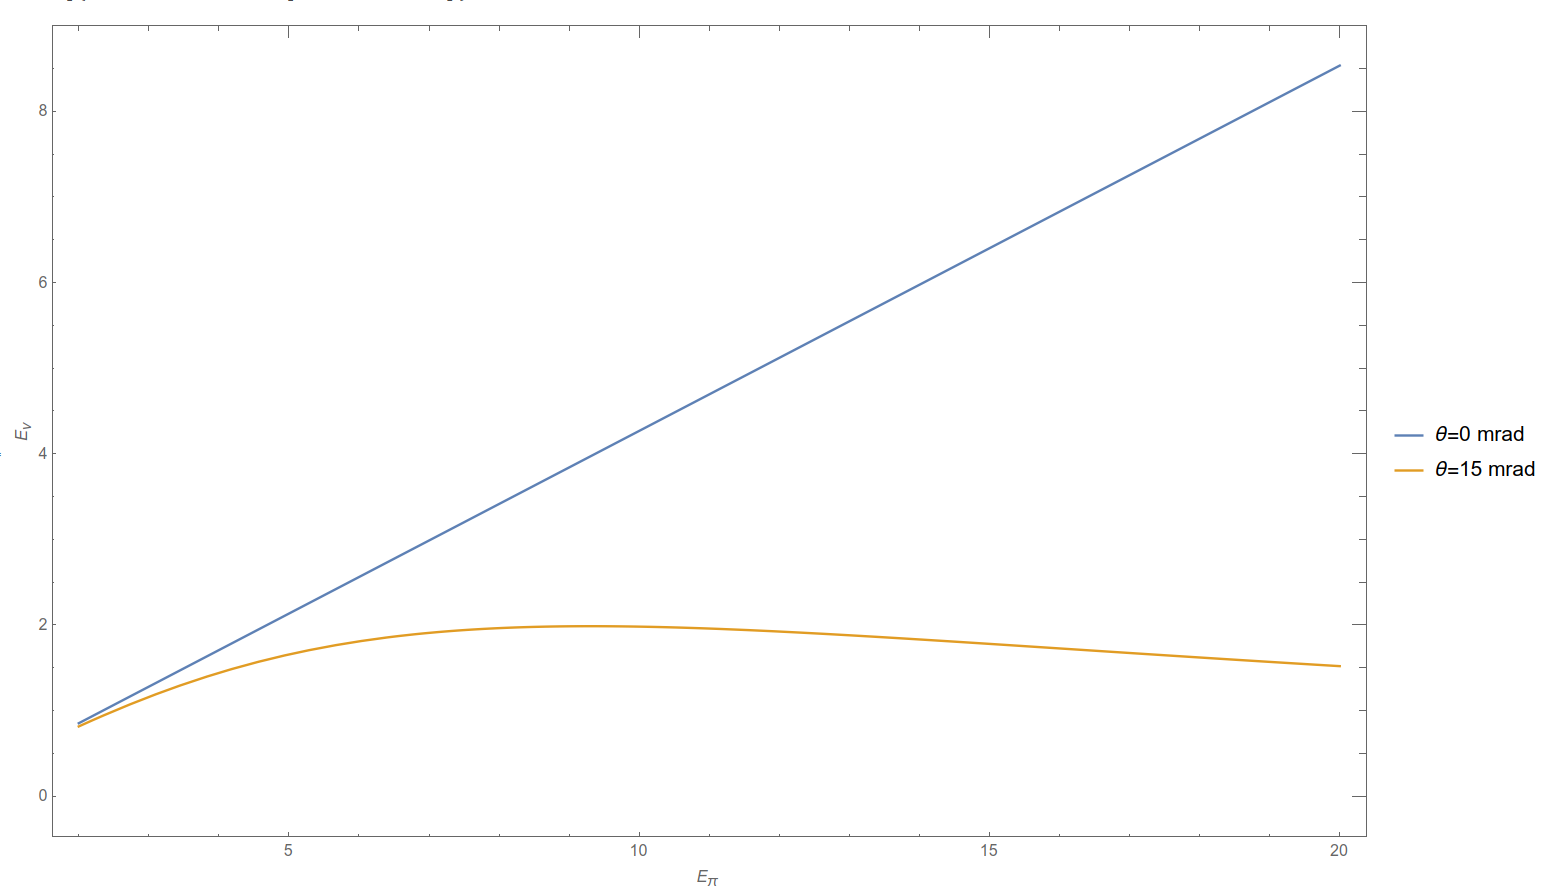
\includegraphics[scale=0.45]{prob3}
		\centering
		\caption{Neutrino energy as a function of pion energy for the decay, $\pi^+\rightarrow \nu_\mu \mu^+$}
		\label{prob3}
		\centering
	\end{figure}

\end{homeworkProblem}

\end{document}

